\documentclass[12pt]{report}

\usepackage[utf8]{inputenc}
\usepackage[IL2]{fontenc}
\usepackage[czech]{babel}
\usepackage{menukeys} 
\usepackage{listings}
\usepackage{lipsum}
\usepackage{mwe}

\usepackage[
	left=30mm, 
	right=30mm, 
	top=40mm, 
	bottom=30mm,
]{geometry}


\usepackage{graphicx}
\graphicspath{{Images/}} 

\usepackage{amsmath}
\usepackage{parskip}
\usepackage[hidelinks]{hyperref}
\usepackage[nottoc]{tocbibind}

\begin{document}
	
\begin{titlepage}
	\centering		
	\Large			
	\sffamily		
	
	
\includegraphics[width=.7\textwidth]{fav}
	
	Semestrální práce z předmětu
	
	Programování v jazyce ANSI C
	
	\vspace{15mm}
	{\Huge\bfseries Identifikace spamu naivním bayesovským klasifikátorem}
	
	\vspace{15mm}
	\today 
	
	\vfill			
	\raggedright	
	\emph{Autor:}\\		
	Václav Tran\\		
	A21B0299P\\
	\texttt{nuva@students.zcu.cz}
	
	\vspace{\baselineskip}
	\emph{Vyučující:}\\
	Ing. Kamil Ekštein, Ph.D.\\
	\texttt{kekstein@kiv.zcu.cz}
\end{titlepage}
	
\tableofcontents

\chapter{Zadání}
\label{sec:zadani}
Naprogramujte v ANSI C přenositelnou {\bfseries konzolovou aplikaci}, která bude {\bfseries rozhodovat, zda úsek textu} (textový soubor předaný jako parametr na příkazové řádce) {\bfseries je nebo není spam}.

Program bude přijímat z příkazové řádky celkem {\bfseries sedm} parametrů: První dva parametry budou vzor jména a počet trénovacích souborů obsahujících nevyžádané zprávy (tzv. {\bfseries spam}). Třetí a čtvrtý parametr budou vzor jména a počet trénovacích souborů obsahujících vyžádané zprávy (tzv. {\bfseries ham}). Pátý a šestý parametr budou vzor jména a počet testovacích souborů. Sedmý parametr představuje jméno výstupního textového souboru, který bude po dokončení činnosti Vašeho programu obsahovat výsledky klasifikace testovacích souborů.

Podrobnější popis viz \cite{zadani}.
\chapter{Analýza úlohy}
\section{Slovník}
\label{sec:slovnik}
Ke klasifikaci textového souboru podle zadání viz \ref{sec:zadani} se nejdříve musí vytvořit vhodná datová struktura, která bude uchovávat všechna slova textového souboru (slovník). Dvě takovéto datové struktury jsou trie a hash tabulka (tabulka s rozptýlenými položkami).

Obě datové struktury jsou poměrně porovnatelné. Amortizovaný čas na vyhledání slova v hash tabulce je $O(k)$, kde $k$ je délka slova (za předpokladu, že byla vybraná vhodná hashovací funkce). Čas na vyhledání slova v trii je také $O(k)$. Výhoda využití trie je to, že nevyžaduje hashovací funkci. V případě, že hash tabulka bude využívat nevhodnou hashovací funkci, trie by byla vhodnější výběr.

V této úloze bude vybrána hash tabulka z důvodu větší znalosti implementace a využití. Na konci této kapitoly jsou uvedeny grafické podoby těchto datových struktur (převzato z \cite{pt}).

\begin{figure}
    \label{img:prikladtrietabulka}
    \centering
    \begin{minipage}{0.5\textwidth}
        \centering
        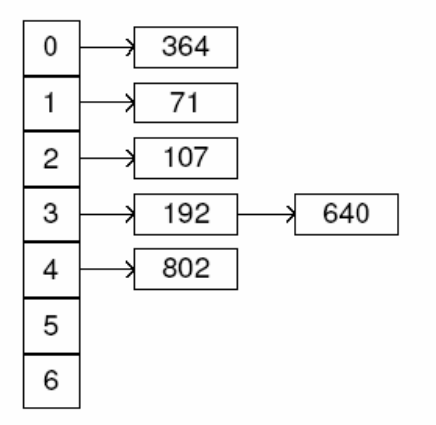
\includegraphics[width=0.9\textwidth]{Images/tabulka.png}
        \caption{Příklad hash tabulky metodou rozptýlených indexů}
    \end{minipage}\hfill
    \begin{minipage}{0.5\textwidth}
        \centering
        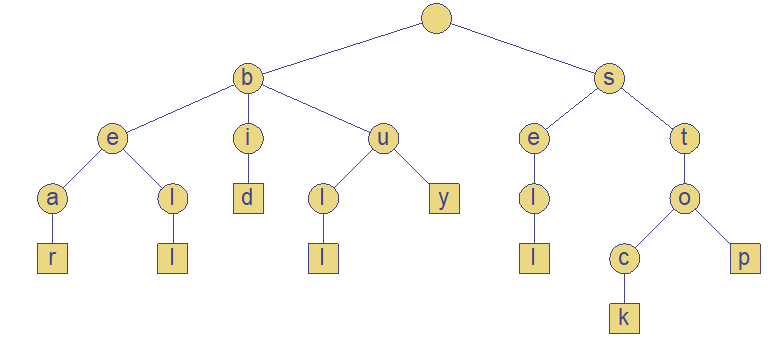
\includegraphics[width=0.9\textwidth]{Images/trie.png}
        \caption{Příklad standardní trie}
    \end{minipage}
\end{figure}

\section{Naivní bayesovský klasifikátor}
Ke klasifikaci bude využit algoritmus popsaný v podrobnějším zadání semestrální práce viz \cite{zadani}. Tento algoritmus bude vyžadovat počet výskytů slova (frekvenci) a vypočítání pravděpodobností $P(c)$ a $P(\langle \text{word} | c \rangle)$, kde 
$c$ je klasifikační třída. V této úloze jsou 2 třídy: $spam$ a $ham$ (pravděpodobnosti jsou podrobněji popsané viz \cite{zadani}). 

Do hash tabulky si v tomto případě nebudeme jenom ukládat slova, ale i jejich frekvenci a pravděpodobnost, že se dané slovo vyskytne v textovém souboru za podmínky klasifikace do třídy $c$. Do hash tabulky si budeme ukládat prvky typu datové struktury $node$, která v sobě bude uchovávat potřebné informace. 
\chapter{Popis implementace}
\section{Hash tabulka}
\subsection{Datové struktury}
Hash tabulka reprezentuje slovník. Využívá metodu rozptýlených indexů (zřetězení) a hashovací funkci ''djb2'' viz \cite{djb2}. Do tabulky se budou ukládat prvky typu $node$, který v sobě uchovává
\begin{itemize}
    \item $key$ - název slova 
    \item $freq$ - počet výskytů slova
    \item $p\_spam$ - pravděpodobnost výskytu slova za podmínky klasifikace do třídy $spam$
    \item $p\_ham$ - pravděpodobnost výskytu slova za podmínky klasifikace do třídy $ham$
    \item $next$ - ukazatel na další prvek typu $node$
\end{itemize}
Samotná hash tabulka je reprezentována datovou strukturou $hashtable$. Tato datová struktura v sobě uchovává
\begin{itemize}
    \item $arr$ - ukazatel na ukazatele na $node$
    \item $kapacita$ - kapacita tabulky
    \item $count$ - počet prvků v tabulce
    \item $uq\_item\_count$ - počet unikátních prvků
\end{itemize}
Při vkládání prvků se vypočítá přes hashovací funkci \textbf{kyblík} (index), do kterého prvek bude patřit. 
\subsection{Vkládání prvků}
V tomto kyblíku se vkládaný prvek bude porovnávat s každým prvkem v tomto kyblíku\footnote{Prvky jsou ekvivalentní pokud obsahují stejné slovo}, aby se zjistilo, zda
tento prvek už v tomto kyblíku není. 

Pokud jsou si prvky rovny, změní se jenom počet výskytů slova. V opačném případě se prvek vloží na konci zřetězení a zvýší se počet unikátních prvků v tabulce. Při každém vkládání prvku (bez ohledu na to, zda prvek v této tabulce již existuje) se navýší počet prvků v tabulce $count$.
\subsection{Udržení složitosti}
Aby se udržela amortizovaná složitost $O(k)$ během vkládání a vyhledávání prvku, musí se zajistit, aby $n/m$ byla konstanta $z$, kde $n$ je počet prvků v tabulce a $m$ je kapacita nebo počet kyblíků v tabulce. 

Pokud $n/m$ přesáhne hodnotu $z$, vytvoří se nový $arr$ s dvakrát větší kapacitou než původní $arr$ a všechny prvky (ukazatelé) původního $arr$ se přesunou do nového $arr$. Je zřejmé, že se v tomto případě navýší i $kapacita$ tabulky.

Toto zajišťuje funkce \verb|rehash()|, která se vykonává při vkládání prvku za podmínek uvedených výše.
\section{Naivní bayesovský klasifikátor}
\subsection{Datové struktury}
Algoritmus pro tento klasifikátor vyžaduje definici množiny a trénovací množiny. K tomuto účelu byla vytvořena datová struktura $set$, která v sobě uchovává:
\begin{itemize}
    \item $dict$ - slovník (hash tabulku)
    \item $dict\_file\_count$ - počet textových souborů, které byly načteny do slovníku
    \item $probability$ - apriorní pravděpodobnost této množiny
\end{itemize}
Pro tento klasifikátor si připravíme 3 množiny:
\begin{enumerate}
    \item $spam$ - obsahuje prvky, patřící do třídy $spam$
    \item $ham$ - obsahuje prvky, patřící do třídy $ham$
    \item $total$ - obsahuje prvky, patřící do třídy $spam$ nebo $ham$
\end{enumerate}
Účely těchto množin je vysvětleno níže v sekci \ref{subsec:trainset}.

Tyto tři množiny se budou uchovávat v datové struktuře $trainset$, která reprezentuje trénovací množinu.
Uchovává v sobě 3 výše uvedené množiny a počet množin v trénovací množině.

\subsection{Načítání textových souborů}
\label{subsec:loadingfile}
Každý soubor musí být zpracovaný a extrahovaná slova ze souboru musí být uložena do daného slovníku. Toto nám zajišťuje funkce \verb|load_words()|.

Funkce \verb|load_words()| načte ale jenom jeden soubor s daným názvem. Pro naše účely je toto nedostatečné, potřebujeme načíst všechny soubory s názvem: \verb|vzorN|, kde~\verb|N| je celé číslo z intervalu $\langle1,N\rangle$ a všechny názvy souborů obsahují příponu ''.txt''. 
Tuto funkčnost nám zajišťují funkce \verb|load_words_from_vzor_files()| a \verb|create_vzor_name()|.

Funkce \verb|create_vzor_name()| vytvoří podle daného řetězce \verb|vzor| a celého čísla \verb|I|~řetězec~\verb|vzorI|. 
Funkce \verb|load_words_from_vzor_files()| pomocí funkce \verb|load_words()| a funkce \verb|create_vzor_name()| má všechny potřebné prvky k tomu, aby načetla všechny slova ze souborů \verb|vzorN.txt| do daného slovníku.

\subsection{Vytváření trénovací množiny}
\label{subsec:trainset}
Vytváření trénovací množiny nám zajišťuje funkce \verb|create_training_set()|.
Pomocí funkcí z \ref{subsec:loadingfile} se naplní tyto 3 vytvořené množiny: $spam$, $ham$ a $total$. V trénovací množině budeme přistupovat k těmto množinám pomocí indexů $0,1,2$. Index reprezentující $spam$ bude $0$, index reprezentující $ham$ bude $1$ a index reprezentující $total$ bude $3$.

U této trénovací množiny ale nastavíme počet prvků v této množině na 2. Důvodem je, že při fázi klasifikace a učení budeme chtít jenom procházet množiny $spam$ a $ham$. K množině $total$ budeme přistupovat manuálně. Důsledkem této vychytávky je, že při uvolňování trénovací množiny pomocí funkce \verb|free_trainset()| se k počtu prvků v trénovací množině musí přičíst 1, aby se uvolnila i množina $total$.

\subsection{Fáze učení a fáze klasifikace}
Fáze učení je reprezentována funkcí \verb|NB_learn_text()| a fáze klasifikace jednoho textového souboru je reprezentovaná funkcí \verb|NB_classify_text()|. Fáze klasifikace pro více souboru je reprezentovaná metodou \verb|NB_classify_vzor_text()|.

Funkce \verb|NB_learn_text()| a \verb|NB_classify_text()| byly vytvořeny podle pseudokódu viz \cite{zadani}.

Funkce \verb|NB_classify_vzor_text()| využívá funkci \verb|create_vzor_name()| k vytvoření vyžadovaných názvů souborů. Všechny tyto textové soubory se klasifikují a vytvoří se výstupní soubor s názvem předaný jako parametr. 

Tento výstupní soubor bude obsahovat klasifikaci jednotlivých souborů ve formátu uvedeným v \cite{zadani}. Ukázka výstupního souboru je také viditelná viz \ref{img:resultxt}.


\chapter{Uživatelská příručka}
\section{Přeložení a sestavení programu}
Pro přeložení a sestavení programu byly vytvořeny 2 \verb|makefile| soubory. 

\verb|makefile.win| je určen pro Windows a \verb|makefile| je určen pro Linux. Uživatelé na~Windows~si navíc budou muset nainstalovat kompilátor jazyka C (např. {\bfseries MinGW} nebo {\bfseries MSVC}). Příkaz pro sestavení programu může vypadat takto:

{\bfseries Windows\footnote{Zde záleží, jaký kompilátor využíváte. V této ukázce se využívá MinGW.}:} 
\begin{lstlisting}[
    mathescape,
    columns=fullflexible,
    basicstyle=\small\fontfamily{lmvtt}\selectfont,
]
    mingw32-make -f makefile.win
\end{lstlisting}
{\bfseries Linux}:
\begin{lstlisting}[
    mathescape,
    columns=fullflexible,
    basicstyle=\small\fontfamily{lmvtt}\selectfont,
]
    make -f makefile
\end{lstlisting}
Po zadání vybraného příkazu se vytvoří soubor \verb|spamid.exe|.
\newpage
\section{Použití programu}
Program by se měl spouštět příkazem:
\begin{lstlisting}[
    mathescape,
    columns=fullflexible,
    basicstyle=\fontfamily{lmvtt}\selectfont,
]
    spamid.exe $\langle$spam$\rangle$$\langle$spam-cnt$\rangle$$\langle$ham$\rangle$$\langle$ham-cnt$\rangle$$\langle$test$\rangle$$\langle$test-cnt$\rangle$$\langle$out-file$\rangle$
\end{lstlisting}
Symboly $\langle$\verb|spam|$\rangle,\langle$\verb|ham|$\rangle$ a $\langle$\verb|test|$\rangle$ představují vzory jména vstupních souborů. Symboly $\langle$\verb|spam-cnt|$\rangle$,$\langle$\verb|ham-cnt|$\rangle$,$\langle$\verb|test-cnt|$\rangle$ představují počty vstupních souborů. 

Symboly $\langle$\verb|spam|$\rangle,\langle$\verb|ham|$\rangle$ určují soubory, ze kterých bude probíhat fáze učení.
Symbol $\langle$\verb|test|$\rangle$ určuje soubory, které se budou klasifikovat do třídy $spam$ nebo $ham$.
Symbol $\langle$\verb|out-file|$\rangle$ zde určuje název výstupního souboru, kde budou uloženy výsledky klasifikace jednotlivých textových souborů.

Soubory klasifikovány do třídy $spam$ představují nevyžádané zprávy. Soubory klasifikovány do třídy $ham$ jsou naopak zprávy, které přijímáme.

Všechny vstupní soubory musí být umístěny v podadresáři \verb|data|. Obsah vstupního souboru by mohl vypadat takto:
\begin{lstlisting}[
    mathescape,
    columns=fullflexible,
    basicstyle=\fontfamily{lmvtt}\selectfont,
]
    hello money rich quick research center content length
\end{lstlisting}
Slova musí být od sebe oddělena právě jednou mezerou.


Vstupní soubory mají následující pojmenování: \verb|vzorN|, kde $\mathrm{N}$ je celé číslo z intervalu $\langle 1 ; N\rangle$. Přípona všech vstupních souborů je .txt, přípona není součástí vzoru. Váš program tedy může být během testování spuštěn například takto:

\begin{lstlisting}[
    mathescape,
    columns=fullflexible,
    basicstyle=\fontfamily{lmvtt}\selectfont,
]
    spamid.exe spam 300 ham 300 test 2 result.txt
\end{lstlisting}
Po vykonání příkazu uvedeného výše může soubor \verb|result.txt| vypadat takto:
\begin{figure}[h]
        \label{img:resultxt}
        \centering
        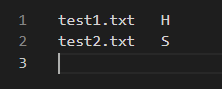
\includegraphics[width=0.5\textwidth]{Images/vysledekpoprikazu.png}
        \caption{Soubor result.txt po vykonání příkazu}
\end{figure}

\chapter{Závěr}
Program správně klasifikuje textové soubory s $>90\%$ úspěšností nad testovacími daty. Zhodnotil bych tudíž splnění zadání jako úspěšné.

Pro správnou klasifikaci při odevzdávání této práce přes validátor se s apriorní pravděpodobností nepočítalo z důvodu nízké správnosti výsledků.

Jeden z možných problémů je malá ''obecnost'' u funkce \verb|create_trainingset()| a funkce \verb|free_trainingset| viz \ref{subsec:trainset}. 
\bibliographystyle{unsrt}
\bibliography{literatura}
\end{document}
